\section{研究内容}
\label{section:研究内容}
観光案内アプリはユーザーが受け取るコンテンツが多いという特徴があるため、パフォーマンスが低下しやすい。~\autoref{subsection:PWAの要素の性質}で示したPWAの構成要素のうち、Service Workerはパフォーマンスの低下を防ぐのに有用であるとされている。そのため、Service Workerを使用した際の観光案内アプリのパフォーマンスを評価する。アプリのパフォーマンスを評価するためには、事前に以下の作業が必要である。
\begin{itemize}
    \item 評価対象となるアプリに求められる機能の調査
    \item 評価対象となるアプリのビルド構成の策定、アプリの作成
    \item Service Workerのキャッシュ戦略の策定
    \item アプリのパフォーマンスを計測する方法の策定
\end{itemize}
\subsection{観光案内アプリに求められる機能の調査}
\label{subsubsection:観光案内アプリに求められる機能の調査}
人々が観光案内アプリと聞いて思い浮かべるものは様々である。そこで、観光案内アプリに求められる機能を調査する。初めにGoogle検索エンジンを使用して都道府県名、「観光」、「アプリ」というキーワードで検索する。次に、最上位の検索結果から順に閲覧していき、観光案内アプリを見つける。そのアプリが配信中であれば、PCやスマートフォンで実際にそのアプリを使用してアプリに実装されている機能を調査する。

初めに、検証用のアプリを作成するために現在配信されている観光案内アプリのうち、モバイルネイティブアプリで実装されている機能を調査した。それぞれの機能とその機能が実装されている割合を降順で表~\ref{table:観光案内アプリに実装されている機能}に示す。パーセンテージは小数第1位を四捨五入している。
\begin{table}
  \caption{観光案内アプリに実装されている機能}
  \label{table:観光案内アプリに実装されている機能}
  \centering
  \begin{tabular}{|p{15em}|p{10em}|}
    \hline
    & 割合[\%] \\ \hline
    観光地図 & 74 \\ \hline
    スタンプラリー & 41\\ \hline
    観光ルート案内 & 33\\ \hline
    観光名所のブックマーク & 26\\ \hline
    Wi-Fiアクセスポイントの検索 & 11 \\ \hline
  \end{tabular}
\end{table}

次に、同様のアプリで使用されているアクセス権限を調査した。それぞれのアクセス権限が使用されている割合とその用途を表~\ref{table:観光案内アプリが使用するアクセス権限とその用途}に示す。パーセンテージは小数第1位を四捨五入している。

\begin{table}
  \caption{観光案内アプリが使用するアクセス権限とその用途}
  \label{table:観光案内アプリが使用するアクセス権限とその用途}
  \centering
  \begin{tabular}{|p{10em}|p{5em}|p{15em}|}
    \hline
    & 割合[\%] & 用途 \\ \hline
    位置情報 & 93 & ユーザーの近くにある観光名所の表示、観光名所のルート案内、観光名所に近づいたときのプッシュ通知の送信 \\ \hline
    プッシュ通知 & 67 & アプリの機能の紹介、観光名所の紹介 \\ \hline
    カメラ & 26 & QRコードの読み取り、観光名所の撮影 \\ \hline
  \end{tabular}
\end{table}
観光地図は、地図レイヤーの上に観光名所などの地点をプロットして表示したものである。プロットされた地点にカーソルを合わせたり、その地点をクリックしたりすると、その地点を説明する画像やテキストが表示される。スタンプラリーは、観光名所などを訪ね、その場所に設置されているビーコンと通信したり、QRコードを読み取ったりすることでスタンプを獲得できる機能である。観光地に設置されているWi-Fiスポットに接続したいユーザー向けに、Wi-Fiアクセスポイントの検索機能を提供しているものもある。

中でも、観光地図を利用する際は観光名所や地図レイヤーの画像が配信されるため、データの通信量が大きくなる。このような場合はService Workerによるキャッシュの恩恵を受けられる。また、実装されている割合が最も大きいため、この機能は多くの観光案内アプリが持つ特徴の1つであると考えられる。観光地図を実装したWebアプリを作成してそのパフォーマンスを計測することで、観光案内アプリにおけるService Workerのパフォーマンスを評価する。
\subsection{評価対象となるアプリの作成}
\label{subsubsection:評価対象となるアプリの作成}
一般的にWebアプリはフレームワークを使用して作成されるため、今回評価対象となるアプリを作成する際もそのソフトウェアを使用する。HTMLの生成方法は大きく分けて2種類あり、どちらを採用するかを決める必要がある。まずは、それらの方法を説明する。

最も基本的なHTMLの生成方法としては動的な生成がある。ユーザーがページにアクセスするたびにサーバー側でHTMLファイルが生成される。動的な生成を使用すると、ユーザーから任意のパラメーターを受け取り、それに基づいてHTMLを生成できる。後述する静的な生成では、Webアプリのプログラムを変更するたびにHTMLを生成し直さなければならないが、動的な生成ではその必要がないため、最新の情報を素早くユーザーに届けられる。動的な生成はSSR(Server Side Rendering)という仕組みによって実現しており、通常、HTMLを動的に生成する場合は、WebサーバーとWebアプリサーバーが必要である。

もう1つの生成方法は静的な生成である。Webアプリを変更してデプロイする際にはビルドという処理が行われるが、静的な生成では、この処理を行う際にそれぞれのページのHTMLファイルが生成される。したがって、ユーザーが特定のページにアクセスした際にクライアントに返却されるHTMLの内容は、ビルドが更新されない限り常に同じである。静的な生成はSSG(Static Site Generator)という仕組みによって実現しており、HTMLを静的に生成する場合はWebサーバーが必要である。

前述したように、静的な生成ではWebアプリのプログラムを変更するたびにHTMLを生成し直さなければならないという短所があり、コンテンツ指向型のWebアプリで静的なHTML生成が用いられることは少ない。そこで、検証用のアプリの作成時はHTMLを動的に生成する方法であるSSRを使用する。

次に観光地図を検証用のアプリに実装する。まずはOpenStreetMap~\cite{OpenStreetMap}を使用して地図レイヤーを表示する。OpenStreetMap(OSM)はコミュニティーによってメンテナンスされている、オープンソースの世界地図および地理データベースである。Overpass APIを使用して、観光名所に分類されるOSMのノードをJSONデータとして取得する。このノードをOSMの世界地図にプロットすることで、観光名所の場所がプロットされた地図を作成できる。Google Mapsに代表されるように、アプリに地図を表示する場合は、ズーム倍率を変更したり、自由にスクロールしたりできるインタラクティブ性が必要である。これを満たすためにLeaflet~\cite{Leaflet}を使用する。観光名所のマーカーにカーソルを合わせたり、そのマーカーをクリックした際に表示される画像やテキストを取得するために、JSONPlaceholderを使用する。JSONPlaceholderは、画像やテキストのダミーデータをREST APIで提供する。通常の観光地図には、特定の地域の観光名所のみがプロットされている。そのため、検証用のアプリでは国内の観光名所を都道府県ごとに表示する。検証用のアプリのスクリーンショットを図~\ref{figure:検証用のアプリのスクリーンショット}に示す。
\begin{figure}
  \centering
  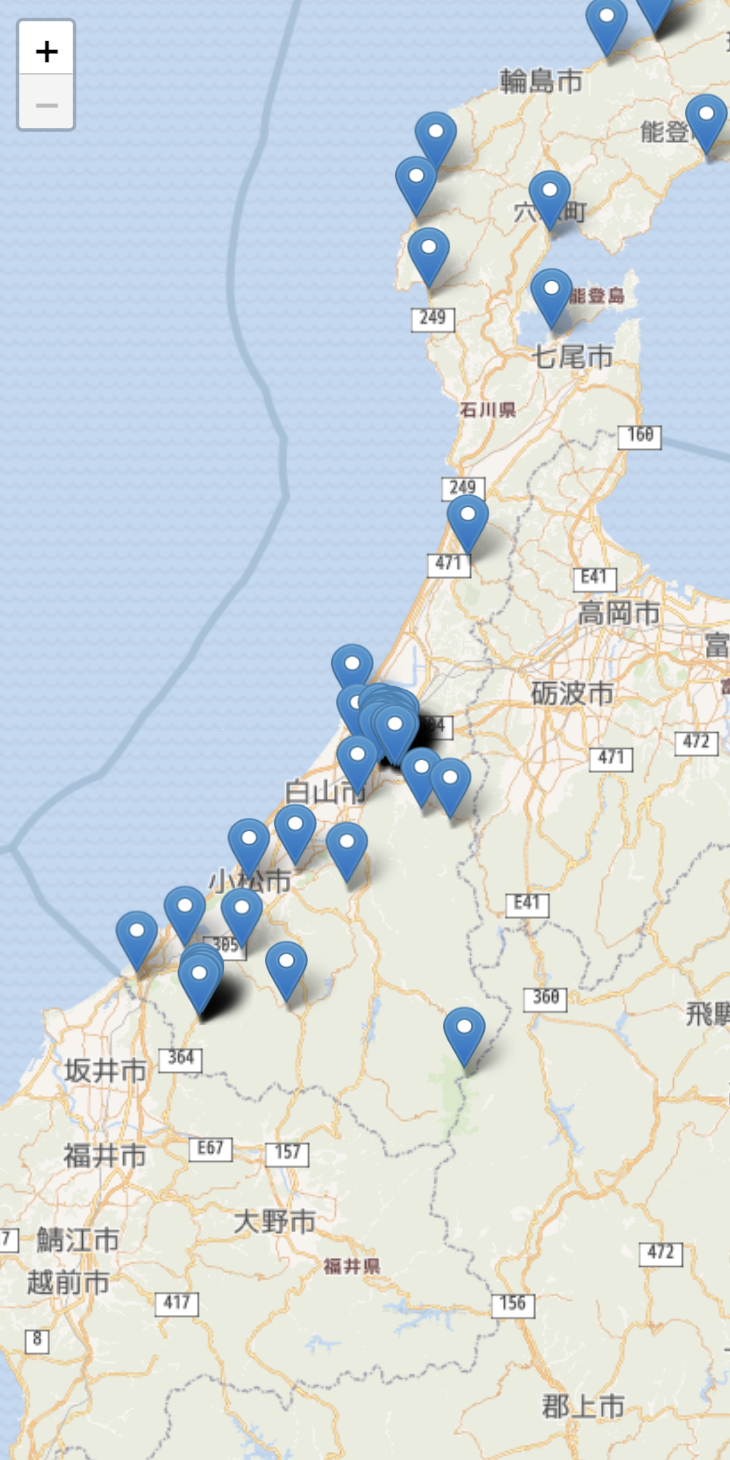
\includegraphics[width=0.5\textwidth]{paper/images/app_screenshot.png}
  \caption{検証用のアプリのスクリーンショット}
  \label{figure:検証用のアプリのスクリーンショット}
\end{figure}

\subsection{Service Workerのキャッシュ戦略}
\label{Service Workerのキャッシュ戦略}
Service Workerのキャッシュ戦略はfetchイベントとCacheインターフェイスからなり、適切なキャッシュ戦略を採用することでPWAのパフォーマンスを向上させられる。Service Workerの処理の流れは以下の通りである。
\begin{enumerate}
    \item ServiceWorkerContainer.register()を使用してService Workerが登録される。登録されたService WorkerはServiceWorkerGlobalScope内で実行される。
    \item installイベントによってService Workerがインストールされる。アプリを完全にオフラインで使用できるようにするための準備が始まる。
    \item 古いバージョンのService Workerによってページが制御されていない場合は、新しいバージョンのService Workerがactivateイベントを受け取る。activateイベントでは、大抵の場合は古いバージョンのService Workerがキャッシュしていたリソースを全て削除する処理が行われる。
    \item Service Workerがfetchイベントを受け取る。fetchイベントでは、リクエストされたリソースの属性やURLに応じて、リソースがService Workerによって制御される。fetchイベントは最初のロードでは発生しないため、Service Workerは2回目以降のロードでリソースを制御する。
\end{enumerate}
どのネットワークレスポンスをキャッシュするべきかはアプリの内容によって異なるため、キャッシュ戦略は無数にあるが、参考までにいくつか例を示す。

まずは、Service Workerのインストール時に全てのアセットをキャッシュする戦略がある。この戦略ではService Workerはアセットのキャッシュのみを返すため、HTMLなどのネットワークリクエストはService Workerを経由せず、キャッシュされない。

あるいは、全てのネットワークリクエストをService Workerに経由させる戦略もある。この戦略ではコンテンツは一切キャッシュされないが、常に最新のネットワークレスポンスを受け取れる。しかし、ユーザーがオフラインのときはWebアプリが機能しない。

このように、Service Workerはネットワークリクエストを仲介する役割を持つ。そのため、Service Workerを用いて一部のコンテンツのみをキャッシュすることもできる。キャッシュ対象のコンテンツの種類や範囲を変化させることでSerivce Workerのパフォーマンス評価を行うことにし、3種類のキャッシュ戦略を策定した。

1つ目はすべてのネットワークレスポンスをキャッシュする戦略である。この戦略では、HTML、CSS、JavaScript、画像、JSONなどのあらゆるネットワークレスポンスがService Workerによって全てキャッシュされる。同じページがもう1度読み込まれると、全てのネットワークレスポンスがキャッシュを利用するため、実質的にネットワークリクエストが発生しない。

2つ目はSame-Originのネットワークレスポンスをキャッシュする戦略である。この戦略ではWebアプリがデプロイされているドメイン(Same-Origin)に対するネットワークリクエストのみがキャッシュされる。同じページがもう1度読み込まれると、Same-OriginのネットワークレスポンスはCache Storageにあるキャッシュを利用し、Cross-Originのネットワークレスポンスはそのキャッシュを利用しない。

3つ目は画像をキャッシュする戦略である。観光案内アプリでは多くの画像が配信されるため、画像を積極的にキャッシュした際のパフォーマンスを知ることは、観光案内アプリでのPWAの有用性を評価する上で重要である。
\subsection{Service Workerのパフォーマンスの計測}
\label{subsection:Service Workerのパフォーマンスの計測}
現在広く普及しているWebアプリの品質測定ツールとしてはLighthouseがある。Lighthouseを使用すると、任意のページに対してパフォーマンス、ユーザー補助、PWA、SEOなどの監査を実施できる。今回はパフォーマンスに着目しているため、パフォーマンスの監査のみを実施する。より正確な指標を得るために、LighthouseのNodeモジュールを使用してモバイル端末での読み込みをエミュレートする。

LighthouseはChrome DevTools Protocol(CDP)というプロトコルを利用している。このプロトコルはプログラムからGoogle Chromeにアクセスできるようにするためのものである。このプロトコルを使用している主なライブラリとしてはchrome-remote-interface、Puppeteer、Ligthouseがある。chrome-remote-interfaceはJavaScriptのAPIを使用してCDPに低レベルでアクセスできる。PuppeteerはCDPの抽象化を提供し、Google Chromeをヘッドレスモードで実行することでWebブラウザーの操作を自動化する。Lighthouseはページのパフォーマンスと品質を改善する方法を見つける処理を自動化するためのライブラリであり、パフォーマンスを評価するために利用できる。

Lighthouseのパフォーマンスの値は0から1で表され、監査項目の条件を満たしているほど、すなわちページの品質が高いほどその値が大きくなる。パフォーマンスの評価に役立つその他の指標としては以下のようなメトリクスがある。

\begin{itemize}
    \item First Contentful Paint(FCP)
    \begin{itemize}
        \item ページのナビゲーションが開始されてから、Webブラウザーがコンテンツの最初の部分をレンダリングするまでにかかる時間である。このコンテンツとはテキスト、画像、<svg>要素、白以外の<canvas>要素を指す。
    \end{itemize}
    \item Largest Contentful Paint(LCP)
    \begin{itemize}
        \item ページのナビゲーションが開始されてから、最も大きな画像またはテキストブロックをレンダリングするまでにかかる時間である。
    \end{itemize}
    \item Speed Index(SI)
    \begin{itemize}
        \item ページの読み込み中にコンテンツが視覚的に表示される速度である。ページを読み込む際に発生するフレーム間の視覚的な変化を計算し、SpeedlineというNodeモジュールを使用して点数を生成する。
    \end{itemize}
    \item Time To Interactive(TTI)
    \begin{itemize}
        \item ページが完全にインタラクティブになるまでの時間である。以下のいずれかの条件を満たした場合は、ページが完全にインタラクティブになったと判定される。
        \begin{itemize}
            \item 最初のコンテンツがレンダリングされること
            \item 視認できるほとんどのページ要素に対してイベントバンドラーが登録されること
            \item ページが50ミリ秒以内にユーザーの操作に応答すること
        \end{itemize}
    \end{itemize}
    \item Total Blocking Time(TBT)
    \begin{itemize}
        \item マクスのクリック、画面のタップ、キーボードの押下などのユーザー入力に対するページの応答がブロックされている合計時間である。
    \end{itemize}
    \item Cumulative Layput Shift(CLS)
    \begin{itemize}
        \item ページの読み込みの開始から終了までの間に発生したセッションウィンドウのうち、そのウィンドウ内のレイアウトシフトの累積値が最も大きいセッションウィンドウの測定値である。
    \end{itemize}
\end{itemize}

モバイル端末をエミュレートする際は、端末の幅、高さ、性能に加えてモバイル端末の通信環境もエミュレートする必要がある。4G以前のモバイル通信システムはIEEE 802.11acなどの広く普及している無線LANの標準規格に比べて通信速度が低いため、無線LANに接続した端末で、ネットワークエミュレーションを行わずにパフォーマンスを計測すると、実際のモバイル端末でのパフォーマンスを正確に計測できない可能性が高い。この問題を回避するためにネットワークスロットリングを使用する。ネットワークスロットリングとはインターネットの速度を意図的に低下させ、低帯域の状態をエミュレートすることである。ネットワークスロットリングには以下の4種類がある。

\begin{itemize}
    \item シミュレートされたスロットリング
    \begin{itemize}
        \item スロットリングされていない最初の読み込みで観察されたデータに基づいてページの読み込みをシミュレートする。高速であるが一部のサイトではスロットリングの正確性が低い。
    \end{itemize}
    \item リクエストレベルのスロットリング
    \begin{itemize}
        \item ネットワークリクエストごとにスロットリングを行う。スロットリングの正確性はSimulated throttlingと同じ程度である。
    \end{itemize}
    \item プロキシーレベルのスロットリング
    \begin{itemize}
        \item HTTPサーバーを経由したTCPやUDPのネットワークリクエストごとにスロットリングを行う。
    \end{itemize}
    \item パケットレベルのスロットリング
    \begin{itemize}
        \item パケットごとにスロットリングを行う。このスロットリングを使用することで最も正確なネットワークシミュレーションを行える。
    \end{itemize}
\end{itemize}

この研究では、より正確なデータを得るために、パケットレベルのスロットリングを使用してパフォーマンスを計測する。パケットレベルのスロットリングを行うためにThrottle~\cite{Throttle}というライブラリを使用する。パフォーマンスを計測する際に使用するネットワークスロットリングのプロファイルを表~\ref{table:ネットワークスロットリングのプロファイル}に示す。
\begin{table}
  \caption{ネットワークスロットリングのプロファイル}
  \label{table:ネットワークスロットリングのプロファイル}
  \centering
  \begin{tabular}{|p{5em}|p{10em}|p{10em}|p{10em}|}
    \hline
    & アップリンク[Kbit/s] & ダウンリンク[Kbit/s] & RTT[ms] \\ \hline
    3gslow & 400 & 400 & 200 \\ \hline
    3gfast & 768 & 1600 & 75 \\ \hline
    4g & 9000 & 9000 & 85 \\ \hline
  \end{tabular}
\end{table}
パフォーマンスの計測からデータの分析までの流れは以下の通りである。
\begin{enumerate}
    \item 予め定義されているスロットリングのプロファイルを用いてネットワークスロットリングを有効にする
    \item Lighthouseを用いてパフォーマンスを計測するプログラムを実行する
    \item csv形式のファイルにLighthouseが収集したデータが記録される
    \item データ分析ツールを用いてそのファイルに記録されたデータを分析する
\end{enumerate}

\subsection{ユーザーの操作に基づいたリソースの読み込みイベントの分析}
\label{subsection:ユーザーの操作に基づいたリソースの読み込みイベントの分析}
Lighthouseはページの読み込みのみを考慮してメトリクスを算出する。観光案内アプリに実装されることが多い観光地図はユーザーの操作に応じて画像を非同期で読み込むため、Lighthouseではそのパフォーマンスを正しく評価できない。そこで、自動テストライブラリの1つであるPuppeteerとResource Timing APIを用いて、観光地図の画像の読み込みイベントを分析する。Resource Timing APIはCSS、JavaScript、画像などのドキュメントに依存するリソースの処理時間を計測する。ネットワークコネクションが終了した後に、Resource Timing APIのコードを実行することで、そのページで読み込まれたあらゆるリソースの処理時間を取得できる。コードの例をソースコード~\ref{lst:Resource Timing APIによるリソースの処理時間の取得}に示す。

\begin{lstlisting}[caption={Resource Timing APIによるリソースの処理時間の取得},label={lst:Resource Timing APIによるリソースの処理時間の取得}]
performance.getEntriesByType('resource');
\end{lstlisting}

この分析では、PerformanceResourceTimingインターフェイスが提供するdurationプロパティーの値を用いて観光地図の画像の読み込み処理にかかった時間を計測する。

リソースの読み込みイベントを分析する際は、~\autoref{subsection:Service Workerのパフォーマンスの計測}の評価方法と同様にネットワークスロットリングを使用して、異なるネットワーク環境における処理時間を計測する。それに加えて、Service Workerの導入による処理時間の変化も計測する。

観光地図の操作パターンの一例として、Google Pixel 5を使用して1ページ下にスクロールする場合と、ズーム倍率を1だけ増加させる場合を考える。